\subsubsection{Testbench và Kết quả mô phỏng Accumulator Register}

\textbf{a. Mô tả Testbench} \\
\begin{itemize}
    \item Kích hoạt tín hiệu \texttt{rst} để kiểm tra sự đồng bộ \texttt{clk}.
    \item Đưa dữ liệu ngẫu nhiên vào ngõ \texttt{D} nhưng tắt tín hiệu \texttt{load\_en} để kiểm chứng chức năng giữ trạng thái cũ.
    \item Bật đồng thời \texttt{load\_en} và \texttt{rst} để kiểm tra mức độ ưu tiên của tín hiệu điều khiển.
\end{itemize}

\textbf{b. Mã nguồn Testbench}
\begin{lstlisting}[language=Verilog, caption={Testbench Accumulator Register}]
`timescale 1ns / 1ps

module tb_Accumulator();

    reg clk;
    reg rst;
    reg load_en;
    reg [31:0] D;
    wire [31:0] Q;

 
    Accumulator uut (
        .clk(clk),
        .rst(rst),
        .load_en(load_en),
        .D(D),
        .Q(Q)
    );

   
    always #5 clk = ~clk;

    initial begin
       
        $display("-----------");
        $display("Time|rst|load_en|D(hex)|Q(hex)");
        $display("-----------");
        $monitor("%10t|%b|%b|%h|%h",$time,rst,load_en,D,Q);

       
        clk = 0; rst = 0; load_en = 0; D = 32'h0;

       
        #12; rst = 1;     
        #10.1; rst = 0;    

      
        #10.1; D = 32'hAAAA_5555; load_en = 1; 
        #10.1; load_en = 0;                    
        
      
        #10.1; D = 32'h1234_ABCD;
        #10.1; 

      
        #10.1; load_en = 1;
        #10.1; load_en = 0;

      
        #10.1; D = 32'hFFFF_FFFF; load_en = 1; rst = 1; 
        #10.1; rst = 0; load_en = 0; 

        #20;
        $display("-------------");
        $display("Hoan thanh mo phong Accumulator!");
        $finish;
    end

endmodule
\end{lstlisting}

\textbf{c. Sơ đồ mạch RTL (RTL Schematic)} 

\begin{figure}[H]
    \centering
    % Thay 'acc_rtl_schematic.png' bang ten file anh so do mach cua ban
    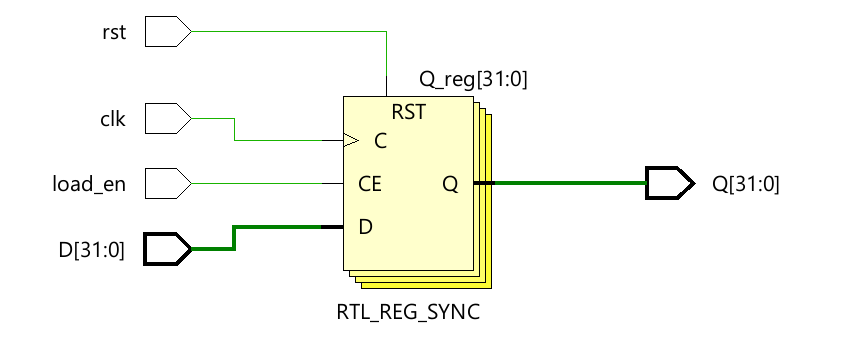
\includegraphics[width=0.7\textwidth]{machacc.png} 
    \caption{Sơ đồ mạch RTL của khối Accumulator}
    \label{fig:acc_rtl}
\end{figure}

\textbf{d. Kết quả xuất ra màn hình}

\begin{figure}[H]
    \centering
    % Thay 'acc_console.png' bang ten file anh console cua ban
    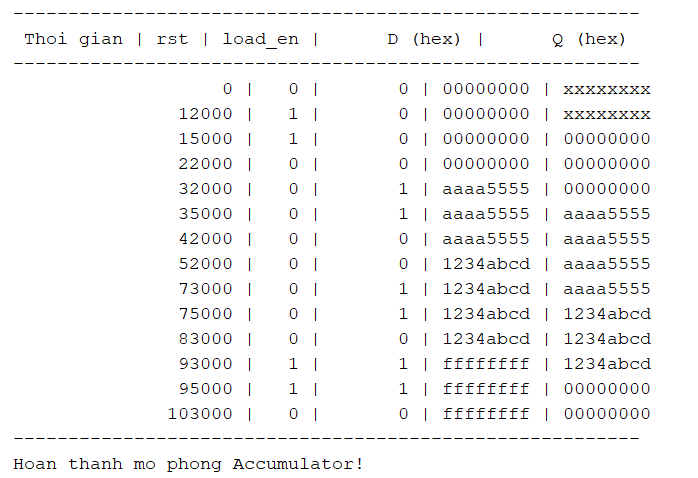
\includegraphics[width=0.8\textwidth]{consoleaccum.png} 
    \caption{Kết quả chạy Testbench Accumulator trên Console}
    \label{fig:acc_console}
\end{figure}

Ngõ ra \texttt{Q} chỉ phản hồi với ngõ vào \texttt{D} khi có lệnh \texttt{load\_en}. 
Trong trường hợp cả \texttt{rst} và \texttt{load\_en} cùng ở mức cao, 
thanh ghi lập tức ưu tiên đưa dữ liệu về mức \texttt{0}, tuân thủ đúng mức ưu tiên trong cấu trúc \texttt{if-else}.

\textbf{e. Giản đồ sóng}

\begin{figure}[H]
    \centering
    % Thay 'acc_waveform.png' bang ten file anh waveform cua ban
    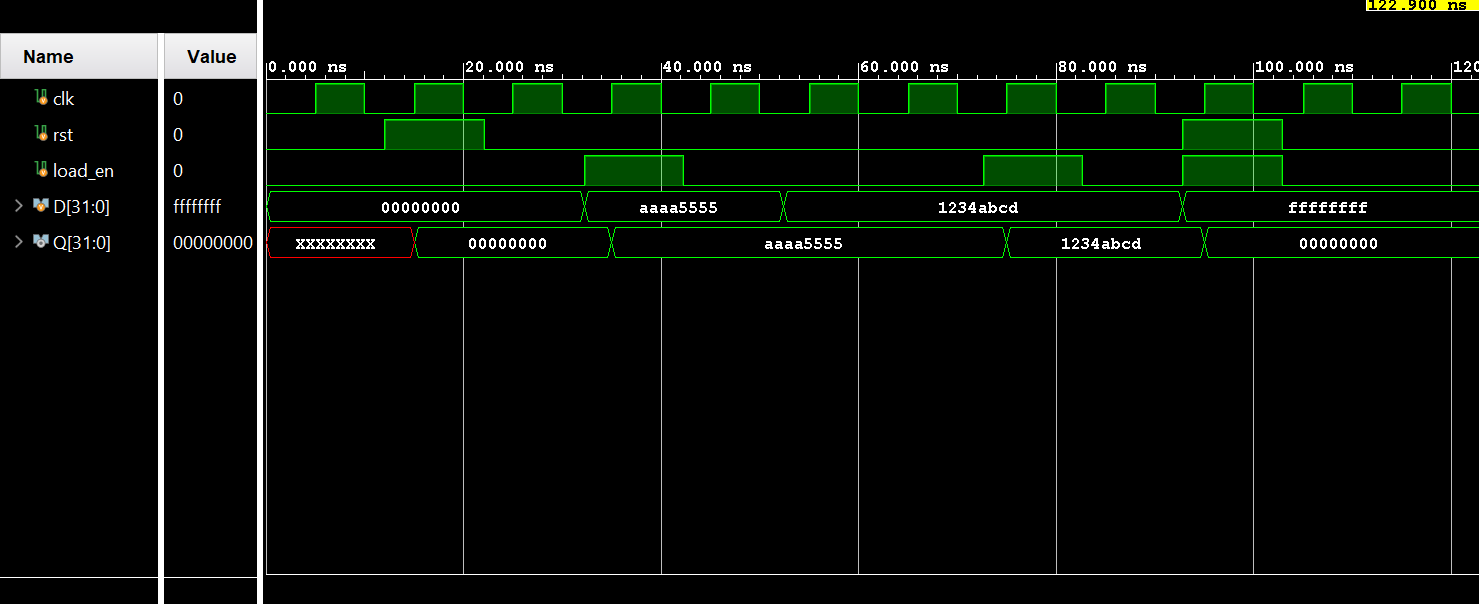
\includegraphics[width=\textwidth]{waveacc.png} 
    \caption{Giản đồ sóng mô phỏng khối Accumulator}
    \label{fig:acc_waveform}
\end{figure}

